%--------------------------------------------------------------
% thesis.tex 
%--------------------------------------------------------------
% Laurea Magistrale in Data Science, Calcolo Scientifico 
% & Intelligenza Artificiale
% https://www.dscsia.unifi.it
% @Scuola di Scienze Matematiche, Fisiche e Naturali
% @Universit\`a degli Studi di Firenze
%--------------------------------------------------------------
% - template for the main file of the LM-DATA@Unifi Thesis 
% - based on Classic Thesis Style Copyright (C) 2008 
%   Andr\'e Miede http://www.miede.de   
%--------------------------------------------------------------
\documentclass[twoside,openright,titlepage,fleqn,
	headinclude,12pt,a4paper,BCOR=5mm,footinclude]{scrbook}
%--------------------------------------------------------------

\newcommand{\myTitle}{Anti-Money Laundering with Graph Neural Networks\xspace}
\newcommand{\myName}{Name Surname\xspace}
\newcommand{\myProf}{prof. Name Surname\xspace}
\newcommand{\myOtherProf}{prof. Name Surname\xspace} %optional: remove this command if the thesis has no co-advisor
\newcommand{\myTime}{Academic Year 2023-2024\xspace}

%--------------------------------------------------------------
\usepackage[english]{babel}
\usepackage[utf8]{inputenc} 
\usepackage[T1]{fontenc} 
\usepackage[square,numbers]{natbib} 
\usepackage[fleqn]{amsmath}  
\usepackage{amsthm}
\newtheorem{definition}{Definition}[chapter]
\usepackage{ellipsis}
\usepackage{listings}
\usepackage{subfig}
\usepackage{caption}
\usepackage{appendix}
\usepackage{siunitx}
%--------------------------------------------------------------
\usepackage{scrhack} % suppress titlesec/tocloft KOMA-Script compatibility warnings
\usepackage{dia-classicthesis-ldpkg}
%--------------------------------------------------------------
% Options for classicthesis.sty:
% tocaligned eulerchapternumbers drafting linedheaders 
% listsseparated subfig nochapters beramono eulermath parts 
% minionpro pdfspacing
\usepackage[eulerchapternumbers,linedheaders,subfig,beramono,eulermath,
parts]{classicthesis}
%--------------------------------------------------------------
\newlength{\abcd} 
\newcommand{\myfloatalign}{\centering} 
\setlength{\extrarowheight}{3pt} % increase table row height
\captionsetup{format=hang,font=small}
%--------------------------------------------------------------
% Layout setting
%--------------------------------------------------------------
\usepackage{geometry}
\geometry{
	a4paper,
	ignoremp,
	bindingoffset = 1cm, 
	textwidth     = 13.5cm,
	textheight    = 21.5cm,
	lmargin       = 3.5cm, % left margin
	tmargin       = 4cm    % top margin 
}

\lstset{
  	frame=tb,
	language=Matlab,
  	aboveskip=3mm,
  	belowskip=3mm,
  	showstringspaces=false,
  	columns=flexible,
  	basicstyle={\small\ttfamily},
  	numbers=none,
  	breaklines=true,
  	breakatwhitespace=true,
  	tabsize=3
}
%--------------------------------------------------------------
\begin{document}
\frenchspacing
\raggedbottom
\pagenumbering{roman}
\pagestyle{plain}
%--------------------------------------------------------------
% Frontmatter
%--------------------------------------------------------------
%--------------------------------------------------------------
% titlepage.tex (use thesis.tex as main file)
%--------------------------------------------------------------
\newcommand{\myDegree}{Laurea Magistrale in Data Science, Calcolo Scientifico \& Intelligenza Artificiale\xspace}
\newcommand{\myUni}{\protect{Universit\`a degli Studi di Firenze}\xspace}
\newcommand{\myLocation}{Firenze\xspace}
\newcommand{\myVersion}{Version 0.1\xspace}
\newcommand{\myFaculty}{Scuola di Scienze Matematiche, Fisiche e Naturali\xspace}
\newcommand{\mySupervisor}{Nome Cognome\xspace}

\begin{titlepage}
	\begin{center}
   	\large
      \hfill
      \vfill
      \begingroup
         
\includegraphics[height=3cm]{LOGO/LOGO_UNIFI}
         \\[.8cm]
	 \myFaculty \\[.2cm]
	 \myDegree \\ 
	\vspace{1cm}    
         \emph{Master Thesis}  
         \vspace{2cm}      
      \endgroup 
      \vfill 
      \begingroup
      	\color{Maroon}\spacedallcaps{\myTitle} \\
	\bigskip
      \endgroup
      \spacedlowsmallcaps{\myName}
      \vfill 
      \vspace{1cm} 
      \vfill
      Advisor: \emph{\myProf}\\[.4cm]
      \ifx\myOtherProf\undefined
      \else
	 Co-Advisor: \emph{\myOtherProf}%
      \fi
      \vspace{1cm}    
      \vfill
      \vfill
      \myTime
      \vfill                      
	\end{center}        
\end{titlepage}   
%--------------------------------------------------------------
% back titlepage
%--------------------------------------------------------------
   \newpage
	\thispagestyle{empty}
	\hfill
	\vfill
	\noindent\myName: 
	\textit{\myTitle,} 
	\myDegree, \textcopyright\ \myTime
%--------------------------------------------------------------
% back titlepage end
%--------------------------------------------------------------
%--------------------------------------------------------------
% abstract.tex (use thesis.tex as main file)
%--------------------------------------------------------------
\chapter*{Abstract}
%--------------------------------------------------------------

Money laundering is estimated to account for between 2\% and 5\% of global GDP annually, yet less than 1\% of illicit financial flows are successfully detected. As criminal organizations increasingly rely on complex, multi-layered transaction networks to obfuscate the origin of illicit funds, traditional rule-based and tabular machine learning approaches prove insufficient: they treat each transaction in isolation, ignoring the rich relational structure that characterizes fraudulent behavior.

This dissertation investigates the use of Graph Neural Networks (GNNs) for the automated detection of money laundering in financial transaction graphs. The problem is formulated as an edge-level classification task on the IBM AMLSim HI-Small synthetic dataset \cite{AMLWorld}, and is addressed under two different settings: a binary task distinguishing licit from illicit transactions, and a multiclass task that additionally identifies the specific laundering pattern involved, enhancing the interpretability of the model's predictions.

We propose a model based on the Group-Aware Graph Neural Network (GAGNN) architecture \cite{mainpaper}, which augments standard GNN backbones with an eMRF smoothing layer and a group representation layer that explicitly clusters accounts suspected of committing money laundering toghether. A multi-task loss combining node-level, edge-level, and group-level objectives is used to jointly optimize detection at all three levels. Two backbone variants are evaluated: one based on Graph Attention Networks (GAGNN-GAT) and one based on Graph Isomorphism Networks (GAGNN-GIN). Both are compared against the corresponding standard GNN baselines without the group-aware components.

The goal of the dissertation is to evaluate GIN as backbone for the GAGNN architecture and to understand whether the GAGNN architecture brings improvements in terms of precision, recall, F1-Score and ROC-AUC compared to baseline GNN models, either on the binary and on the multiclass task.


\pagestyle{scrheadings}
%--------------------------------------------------------------
% Mainmatter
%--------------------------------------------------------------
\pagenumbering{arabic}
% use \cleardoublepage here to avoid problems with pdfbookmark
\tableofcontents
\listoffigures
\cleardoublepage
\thispagestyle{empty}
\begin{flushright}
\null\vspace{\stretch {1}}
\emph{"Citation" \break --- citation's author} \vspace{\stretch{2}}\null
\end{flushright}
\cleardoublepage
%--------------------------------------------------------------

\chapter{Introduction}\label{intro}
Money laundering is the criminal process of disguising or concealing the origin, identity, and ownership of illegally acquired funds.
Its detection has become a foundational pillar of modern economic security.
The rapid digitization of financial services has opened new possibilities for fraudulent activities.
Undetected ML leads to massive economic losses for individuals and institutions, undermines the public trust in the financial system and frequently serves to finance criminal organizations.
The scale of this phenomenon is staggering: the United Nations Office on Drugs and Crime estimates that between 2\% and 5\% of global GDP is laundered annually, with less than 1\% of these illicit financial flows being successfully detected~\cite{unodc2011estimating,europol2016does}.
According to the Canadian Anti Fraud Centre, 704 million dollars were lost because of frauds in 2025 only, confirming the raising trend of the previous years \cite{cafc_home}. 
Consequently, developing robust mechanisms to identify and stop it is critically important to preserving both market integrity and social stability.

The goal of this dissertation is to evaluate the effectiveness of Graph Neural Network (GNN) based models on detecting money laundering patterns. Both precision and explainability will be taken into account and we will propose two different tasks; a binary classification to label transactions as licit or illicit, and a multiclass classification to detect the specific type of laundering strategy employed which, in case of succes, will enhance the explainability of the model. 

In particular we will focus on the Group Aware Graph Neural Network (GAGNN) architecture proposed in \cite{mainpaper}. GAGNN is a GNN-based model that leverages a multi-component loss function to predict if a transaction is licit or illicit. There are a total of 3 losses, a node loss, an edge loss and a group loss. The group one is the novelty of the proposal since it introduces the concept of community by grouping nodes that are suspected to be doing money laundering toghether. More details on the architecture will be provided in Section \ref{sec:gagnn}. 
We will investigate the following inquiries;
\begin{itemize}
    \item whether the GAGNN architecture outperforms other baseline models on the binary task;
    \item whether the GAGNN architecture could be improved by enhancing Graph Isomorphism Network (GIN) instead of Graph Attention Network (GAT);
    \item whether the GAGNN architecture could perform well also on the multiclass task.
\end{itemize}

\section{Structure of the Dissertation}
The dissertation is organized as follows.

\textbf{Chapter~\ref{background} --- Background.}
This chapter lays the theoretical foundations of the work. It begins by introducing the mechanics of money laundering, covering smurfing, fraud rings, and the eight structural laundering patterns, together with an overview of the applicable regulatory framework and the ethical issues that arise when deploying machine learning models in the financial domain. The chapter then motivates the graph-based formulation of the problem, introduces the field of Graph Machine Learning, and formalizes the message-passing framework underpinning GNNs. Two specific architectures are described in detail: Graph Attention Networks (GAT, Section~\ref{sec:gat}) and Graph Isomorphism Networks (GIN, Section~\ref{sec:gin}), followed by a discussion of their theoretical limitations (Section \ref{sec:mp_limits}).

\textbf{Chapter~\ref{approaches} --- Methodology.}
This chapter presents the proposed approach. It describes the Group-Aware Graph Neural Network (GAGNN) architecture, detailing each component of its pipeline: the community-centric encoder, the eMRF layer, the node-level classifier, the group representation layer, and the multi-task loss.
Then it proceeds by providing the description of the \textit{IBM AMLSim Small} dataset used in this work, toghether with his features distributions.
Finally, it covers the experimental setup, including data preparation, the train/validation/test split strategy, subgraph sampling, and the two-phase model selection procedure used to tune both the loss function hyperparameters and the architectural ones.
\textbf{Chapter~\ref{results} --- Results.}
This chapter presents and discusses the experimental results. After reporting the outcomes of the model selection phase, the binary and multiclass classification results of the four models (GAGNN-GAT, GAGNN-GIN, baseline GAT, and baseline GIN) are compared using accuracy, precision, recall, F1-Score, and ROC-AUC as metrics. The chapter concludes with a discussion of the limitations encountered during the study.

\textbf{Chapter~\ref{sec:concl} --- Conclusions.}
The final chapter revisits the three research inquiries formulated above, interprets the results in light of the theoretical properties of the models, and outlines the most promising directions for future work.

%--------------------------------------------------------------
% moneyLaundering.tex (use thesis.tex as main file)
%--------------------------------------------------------------
\chapter{Financial Crime and Money Laundering}
\label{moneyLaundering}
%--------------------------------------------------------------
Understanding how money laundering works is fundamental to garantee both an effective and explainable detection of suspicious transaction. 
This chapter offers a theoretical introduction to money laundering providing a mathematical formulation of the problem together with a summary of common strategies employed by criminals to avoid detection.
\section{The Limitations of the Lonely Scammer}
Individual scammers typically rely on simple and intuitive techniques to introduce illicit funds into the legitimate economy. One of the most prevalent methods is known as ``smurfing''. In simple terms, smurfing involves breaking down a large sum of illicit money into many smaller, inconspicuous chunks to deposit them without raising suspicion. 

More formally, individual scammers rely on smurfing to avoid Anti-Money Laundering (AML) detection mechanisms, which usually flag transactions above a specific threshold $\tilde{x}$. By splitting their initial illicit funds $x$ into smaller transactions $x_n$, such that each transaction satisfies $x_n \leq \tilde{x}$, they minimize the risk of detection \cite{contreras2026strategic}. The mathematical expectation of profit $\pi_s$ for a scammer engaging in smurfing can be defined as:
\begin{equation}
    \pi_s = x(1-\nu)
\end{equation}
where $x$ represents the total initial illicit funds, and $\nu \in (0,1)$ is the friction cost or commission proportion associated with the smurfing process (e.g., the fee paid to mules). 

While smurfing is effective for small amounts, its scalability is severely limited. When attempting to launder much larger volumes of funds, an individual scammer operating from a single account faces a significantly higher probability of detection $(1-p)$, where $p$ is the probability of successfully avoiding detection. If caught, the scammer is subjected to a severe monetary penalty $T$, which includes both the total confiscation of the funds and associated judicial fines \cite{contreras2026strategic}. Therefore, operating as a ``lonely scammer'' becomes mathematically and practically unviable for large-scale operations due to the massive expected cost of $(1-p)T$.

\section{Fraud Rings}
In regard to overcome those issues, criminals have improved their techniques by employing highly sophisticated obfuscation tactics. Instead of acting alone, they form complex ``fraud rings'' to distribute illicit funds across vast networks of temporary accounts. To further break the traceable link between sender and receiver, illicit actors frequently use cyclic transfers and cryptocurrency \textbf{mixers} services that pool together funds from multiple users, mix them, and redistribute them at random intervals and amounts. These advanced tactics create dense, highly camouflaged transaction topologies that easily evade threshold-based rules and simple heuristic detection methods.

To achive their goal they utilize a strategy of transaction layering, often characterized by a topological depth $L$, and network diversification to obscure the money trail \cite{contreras2026strategic, li2025scamsweeper}.
By spreading the funds through a complex topology, the fraud ring successfully increases its non-detection probability $p_L$, which now depends explicitly on the layering depth $L$. The expected profit of a fraud ring utilizing $L$ layers can be mathematically expressed as:
\begin{equation}
    E[\pi_L] = p_L x - (1-p_L)T - c(L)
\end{equation}
where $E[\pi_L]$ is the expected profit, $p_L$ is the enhanced probability of evading detection when $L$ layers are used, $x$ is the total illicit funds, $T$ is the total penalty if caught, and $c(L)$ represents the monotonic cost function associated with establishing and maintaining the $L$ transaction layers. Because the fraud ring dramatically increases the probability of evading detection ($p_L \to 1$ as $L$ increases), the expected payoff remains highly profitable even when factoring in the complex layering costs $c(L)$ \cite{contreras2026strategic}. 

\section{Money Laundering patterns}
Understanding the structural patterns that criminality assumes is fundamental to develop effective detection models and to employ strategies to enhance the explainability of them. According to the literature, there are 8 different patterns that are often used in ML \cite{AMLSim, AMLWorld}. 
\begin{figure}
    \centering
    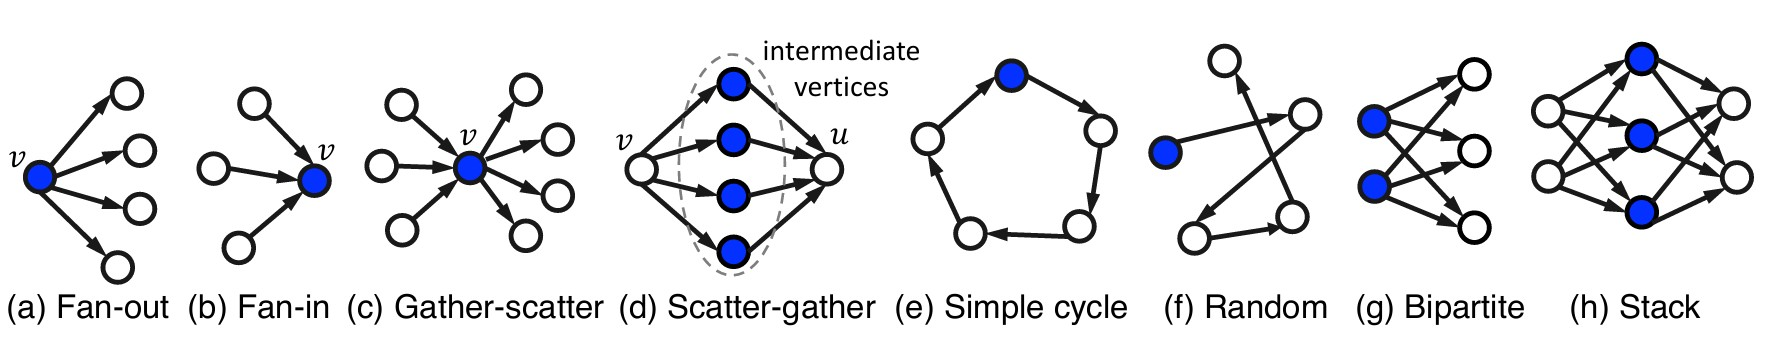
\includegraphics[width=1\textwidth]{IMG/laundering_patterns.jpg}
    \caption{Money Laundering patterns}
    \label{fig:launderingPatterns}
\end{figure}
Which are: 
\begin{itemize}
    \item \textit{fan-out}, shown in Figure \ref{fig:launderingPatterns} a, characterized by outgoing edges from a node $v$ to more than 2 adjacent nodes; 
    \item \textit{fan-in}, Figure \ref{fig:launderingPatterns} b, $v$ is connected to more than 2 nodes by incoming edges;
    \item \textit{gather-scatter}, Figure \ref{fig:launderingPatterns} c, is the combination of a fan-in and a fan-out pattern on the same node $v$;
    \item \textit{scatter-gather}, Figure \ref{fig:launderingPatterns} d, also composed by a fan-in and a fan-out pattern but on two different nodes, sharing the same intermediate neighbors;
    \item \textit{simple-cycle}, Figure \ref{fig:launderingPatterns} e, characterized by a sequence of transactions that starts and ends at the same node;
    \item \textit{random}, Figure \ref{fig:launderingPatterns} f, similar to the cycle but founds do not return to the original account;
    \item \textit{bipartite}, Figure \ref{fig:launderingPatterns} g, moves founds from a set of original nodes to a set of target nodes, with no transactions between accounts of the same set;
    \item \textit{stack}, Figure \ref{fig:launderingPatterns} h, extends the bipartite pattern by adding a second bipartite layer.
\end{itemize}
It's important to mention that in some cases some patterns can be found in both illicit and licit transactions \cite{AMLgentex}. Specifically, \textit{fan-in} and \textit{fan-out} are patterns that are also frequent in legitimate, every-day transactions, such as salary payments or transfers between family members or friends.
That being said, the detection of such patterns remains a foundamental component of any money laundering detection models, albeit insufficient on its own.
Furthermore, a model that correctly classifies those patterns provides a much more interpretable result than one that simply performs a binary classification between licit and illicit transactions. In Chapter \ref{ethics_privacy_regulations} we will see why explainability is of fundamental importance in the financial field. 


\include{Sections/ethics-privacy-regulations}
%--------------------------------------------------------------
% stateOfTheArt.tex (use thesis.tex as main file)
%--------------------------------------------------------------
\chapter{State of the Art}
%--------------------------------------------------------------

\chapter{Task}
In this dissertation we consider the problem of Edge-Level ML detection. This means, considering the Graph $G = (V, E)$ as in Definition \ref{financialGraph}, trying to learn a function \(f\) that, for each transaction $e \in E$, predicts its class. In particular we will consider two different settings. A binary classification where each edge is labeled as fraudulent or lecit and a multi-class classification where, in case of illicit transaction, we also predict the type of pattern, amongst the one described in Section \ref{mlpatterns}, it's involved in.

Formally we seek a function \(f\) that minimizes the error \(L(f)\) over a distribution \(\mathcal{D}\) of Graphs.
\begin{equation}
    \operatorname{argmin}_{f \in \mathcal{H}} \left\{L(f) \doteq \mathbb{E}_{(x,y) \sim \mathcal{D}} [l(f(x), y)]\right\}
\end{equation}
Practically there's no way to know \(\mathcal{D}\). Instead we will consider a dataset \(G_D = (V_D, E_D)\), where both nodes and edges are equipped with feature vectors and we will seek a function \(f\) that minimizes \(L(f)\) over this dataset computing the empirical risk:
\begin{equation}
    \operatorname{argmin}_{f \in \mathcal{H}} \left\{\hat{L}(f) \doteq \frac{1}{|E_D|} \sum_{e \in E_D} l(f(x_e), y_e)\right\}
\end{equation}
This is just the theoretical overview of the problem. In Chapter \ref{approaches} we will provide more insights on how to define the hypothesis space \(\mathcal{H}\) and the loss function \(l\). 

As mentioned in Chapter \ref{ethics_privacy_regulations}, the strict privacy regulations that governs the financial world, makes it hard to find real-world datasets. In this dissertation, for the reasons explained in Section \ref{patterns}, we will use the synthetic dataset \textit{IBM AMLSim}. This is perfect for our scope, since it provides edge lables for both binary and multiclass classification.

\section{Dataset description}
The IBM AMLSim dataset comes in 6 different versions.
\begin{itemize}
    \item HI-Small
    \item HI-Medium
    \item HI-Large  
    \item LO-Small
    \item LO-Medium
    \item LO-Large
\end{itemize}
Where HI (High) and LO (Low) indicate the frequency of illicit transactions and the suffixes Small, Medium and Large indicate the size of the dataset. Figure \ref{fig:datasetstats} shows the differences between the 6 datasets.
\begin{figure}
    \centering
    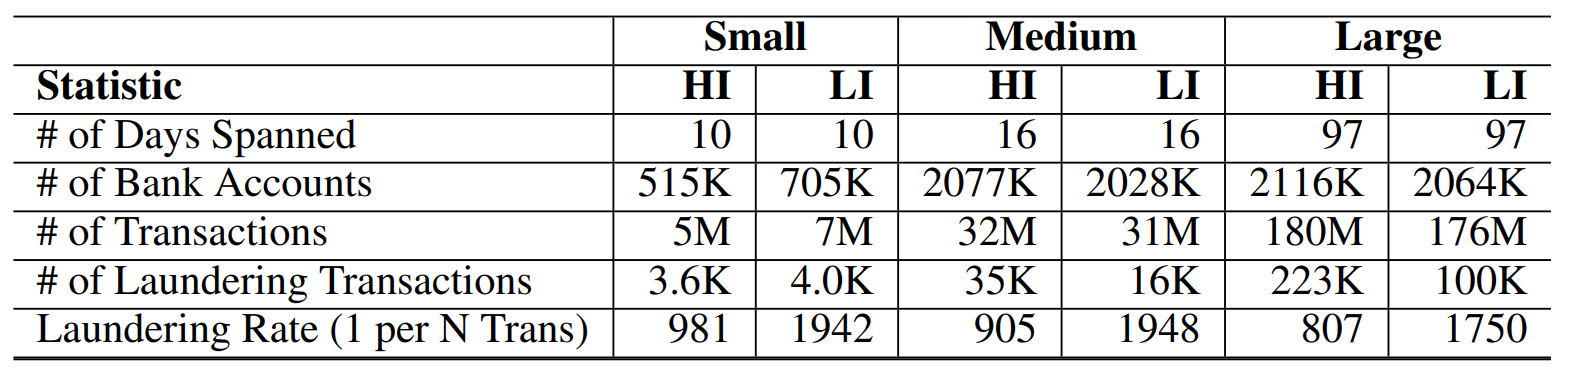
\includegraphics[width=1.0\textwidth]{IMG/dataset.png}
    \caption{IBM AMLSim datasets statistics \cite{AMLWorld}}
    \label{fig:datasetstats}
\end{figure}

In this work we will use the HI-Small version. Bigger datasets would of course garantee a better generalization and accuracy but, for hardware and time constraint, it would be impossible to train the models on such graphs. That begin said, we belive that the obtained results are good enough to understand how the models would perform in a real world scenario.

The HI-Small dataset is composed of 3 different files:
\begin{itemize}
    \item \texttt{HI-Small\_account.csv}, contains 518,581 accounts toghether with their features:
    \begin{itemize}
        \item \textit{Entity ID}: The ID of the account;
        \item \textit{Entity Name}: The name of the account;
        \item \textit{Bank Name}: The name of the bank holding the account; 
        \item \textit{Bank ID}: The ID of the bank holding the account;
        \item \textit{Account Number}: The number of the account;    
    \end{itemize}
    Figure \ref{fig:accountshead} shows some examples of account records.
    \item \texttt{HI-Small\_Trans.csv}, contains transactions features and binary labels:
    \begin{itemize}
        \item \textit{Timestamp}: The timestamp of the transaction;
        \item \textit{From Bank}: The ID of the sending bank;
        \item \textit{From Account}: The ID of the sending account;
        \item \textit{To Bank}: The ID of the receiving bank;
        \item \textit{To Account}: The ID of the receiving account;
        \item \textit{Amount Received}: The amount of money received by the recipient;
        \item \textit{Receiving Currency}: The currency of the received amount (USD, EUR, etc.);
        \item \textit{Amount Paid}: The amount of money paid by the sender;
        \item \textit{Payment Currency}: The currency of the paid amount;
        \item \textit{Payment Format}: The format/method of the payment;
        \item \textit{Is Laundering}: Binary label indicating whether the transaction is illicit;
        \item \textit{src}: Source node identifier;
        \item \textit{dst}: Destination node identifier;
    \end{itemize}
    Figure \ref{fig:transhead} shows some examples of transaction records.
    \item \texttt{HI-Small\_Patterns.txt}, lists the edges that are involved in ML activities toghether with the type of pattern they are involved in (multiclass labels).
    Examples of the 8 differt types of ML patterns in IBM AMLSim are shown in Figure \ref{fig:patternsIBM}.
\end{itemize}
\begin{figure}
    \centering
    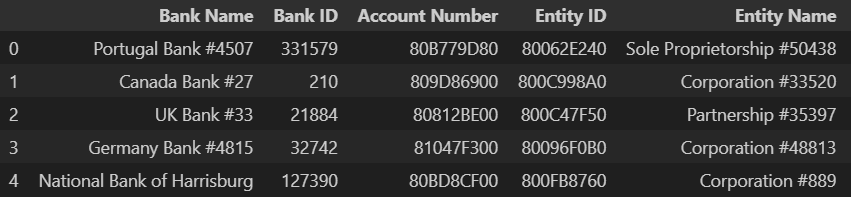
\includegraphics[width=1.0\textwidth]{IMG/accounts_head.png}
    \caption{IBM AMLSim account records}
    \label{fig:accountshead}
\end{figure}
\begin{figure}
    \centering
    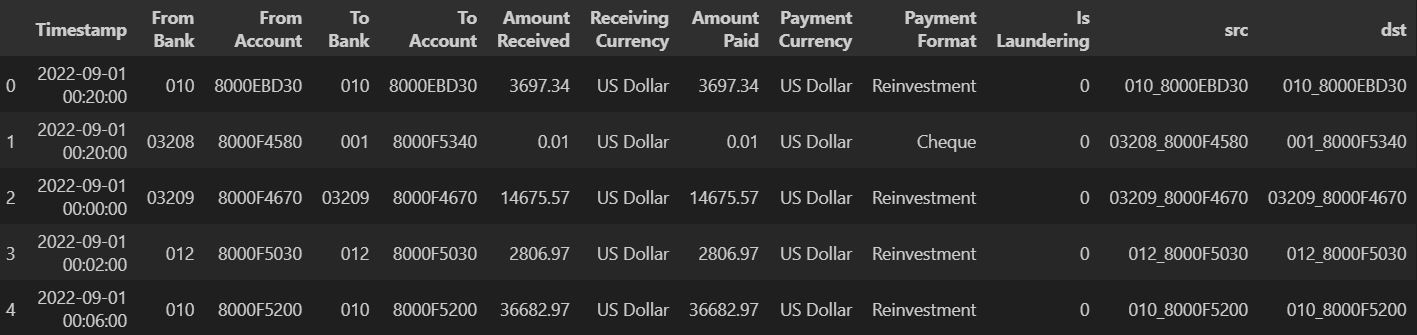
\includegraphics[width=1.0\textwidth]{IMG/trans_head.png}
    \caption{IBM AMLSim transaction records}
    \label{fig:transhead}
\end{figure}
\begin{figure}
    \centering
    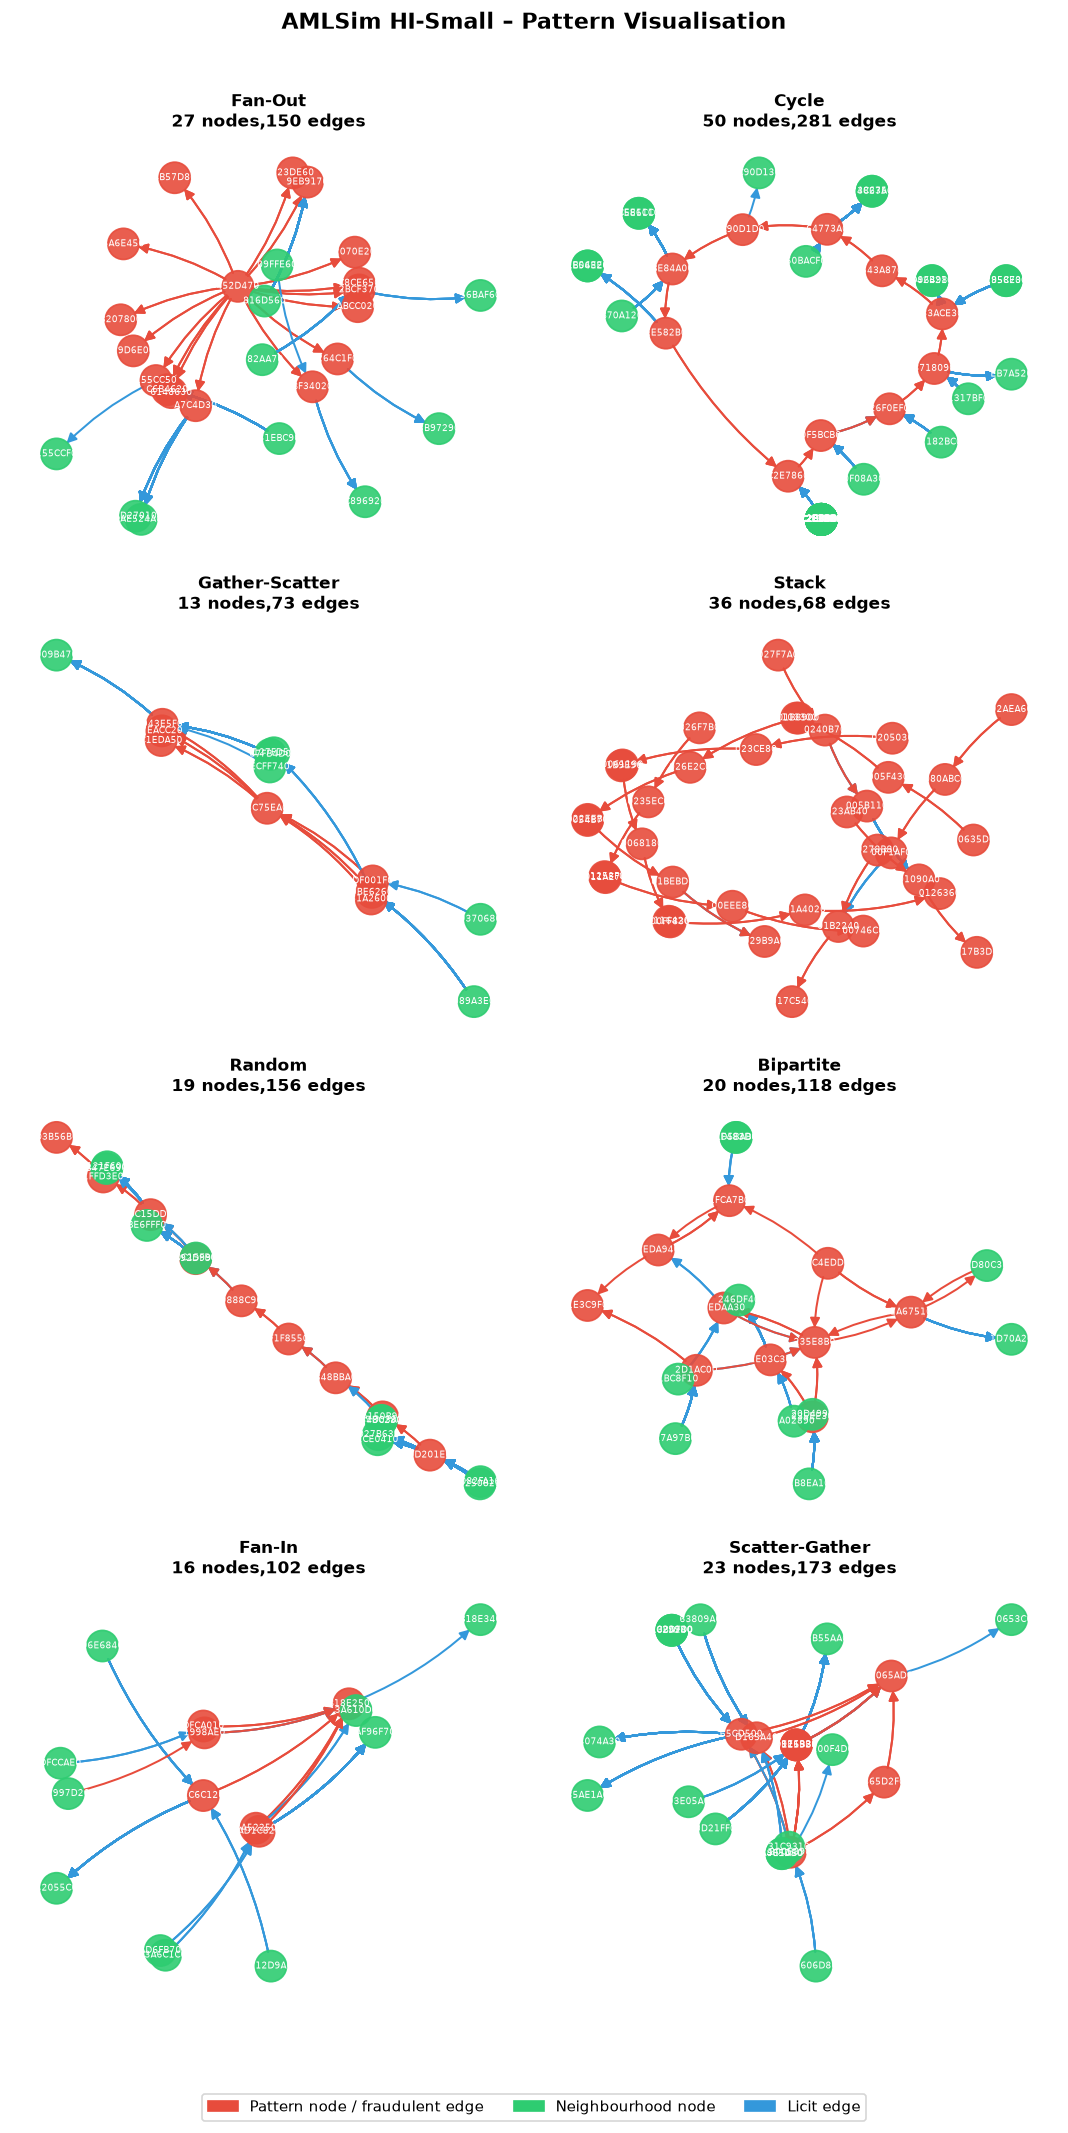
\includegraphics[width=0.76\textwidth]{IMG/patterns.png}
    \caption{IBM AMLSim patterns examples}
    \label{fig:patternsIBM}
\end{figure}
\section{Features analysis}
In this section we provide a detailed analysis of the edges and nodes features distributions. Before diving into that we first take a look at the distribution of the labels in the dataset. There are \(5,177\) illicit transactions over a total of \(5,078,345\) Edges.
Figure \ref{fig:patterns_distr}, provides the distribution of the multiclass label (type of pattern) over the fraudulent edges. It's important to notice that this information is provided only for \(3,149\) out of the \(5,177\) illicit transactions.
\begin{figure}
    \centering
    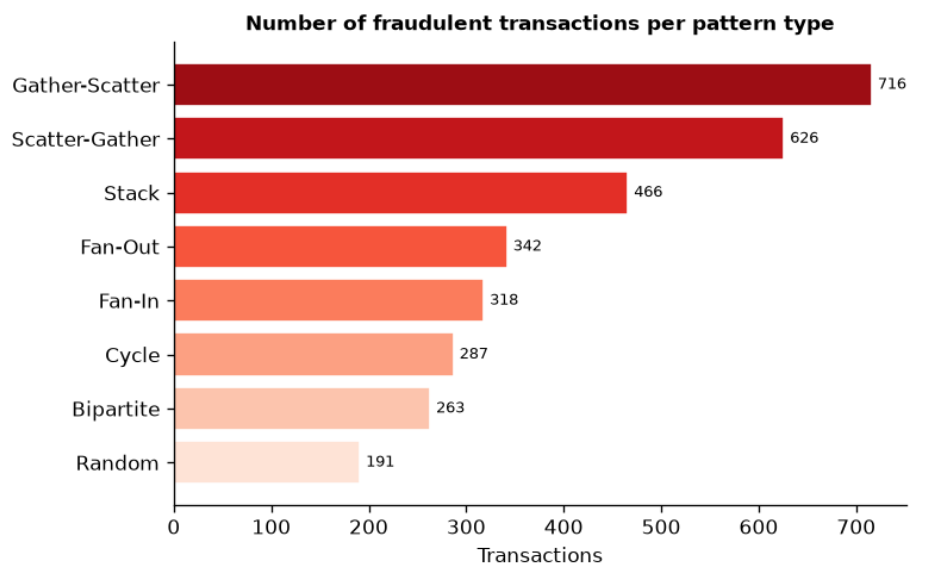
\includegraphics[width=0.8\textwidth]{IMG/patterns_distr.png}
    \caption{IBM AMLSim patterns distribution over fraudulent edges}
    \label{fig:patterns_distr}
\end{figure}

We now procede by analyzing the edge features. First, we notice that \textit{Amount Received} and \textit{Amount Paid} are almost identical. From Figure \ref{fig:amounttrans} we can see that fraudulent trasnactions have the tendency to be bigger than lecit ones.

Continuing our analysis on edge features, we notice that the most common currency is USD for both fraudulent and licit transactions; most of the currencies have a similar proportion distribution from both fraudulent and licit transactions. From Figure \ref{fig:currencytrans} we can see that there are two exceptions: Shekel, which is more prevalent in licit transactions, and Saudi Riyal, which is significantly more prevalent in fraudulent transactions. It's important to notice that the graph shows the proportion of each currency with respect to the total number of transactions in each class; Since there are way more licit than fraudulent transactions, having similar distributions means that, for every type of currency, licit transactions still represent the vast majority.

Considering now the payment formats, by looking at Figure \ref{fig:paymentformats} we notice that ACH transactions are more frequently used for fraudulent transactions compared to other methods.

The last edge feature is \textit{Timestamp}. Since working with timestamps can be tricky, we decided to extract to categorical features representing the hour of the day and the day of the week (Figures \ref{fig:hourday}). Normally we would have also considered the week of the year and the year itself but, since IBM AMLSim Small only covers the span of a week, it would be irrelevant. That being said, it's important to mention that directly working with timestamps, albeit tricky, could lead to a more precise detection [Chapter \ref{futureDirections}]. 
\begin{figure}
    \centering
    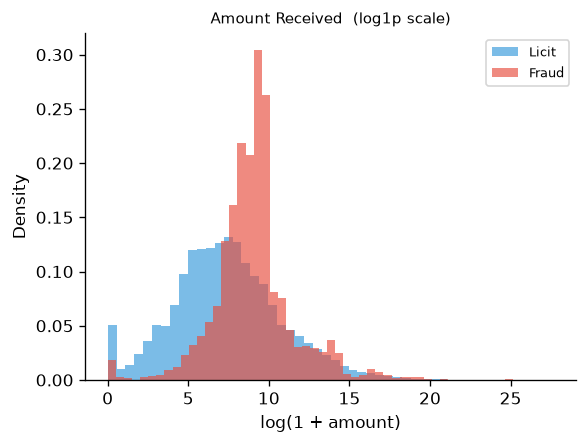
\includegraphics[width=0.8\textwidth]{IMG/amount.png}
    \caption{IBM AMLSim amounts distribution}
    \label{fig:amounttrans}
\end{figure} 
\begin{figure}
    \centering
    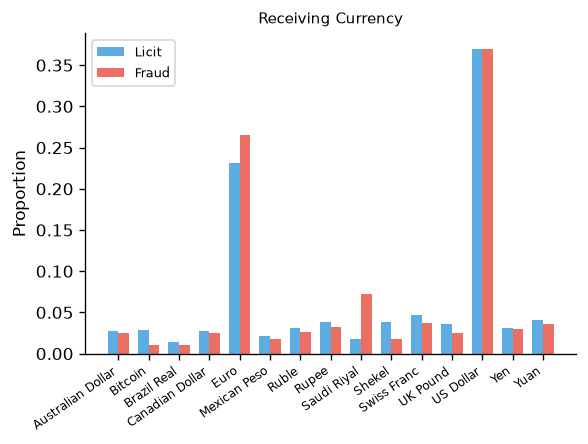
\includegraphics[width=0.8\textwidth]{IMG/currencies.png}
    \caption{IBM AMLSim currencies distribution}
    \label{fig:currencytrans}
\end{figure} 
\begin{figure}
    \centering
    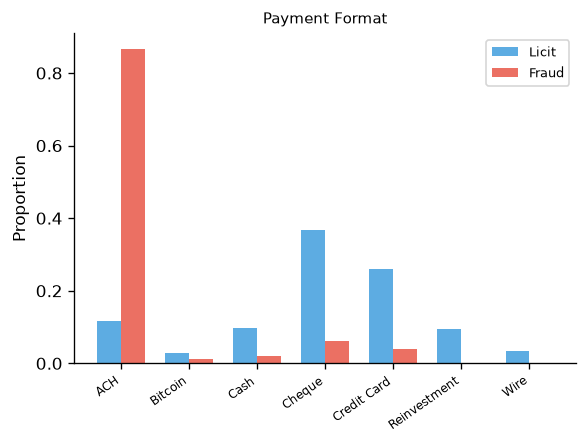
\includegraphics[width=0.8\textwidth]{IMG/format.png}
    \caption{IBM AMLSim payment formats distribution}
    \label{fig:paymentformats}
\end{figure} 
\begin{figure}
    \centering
    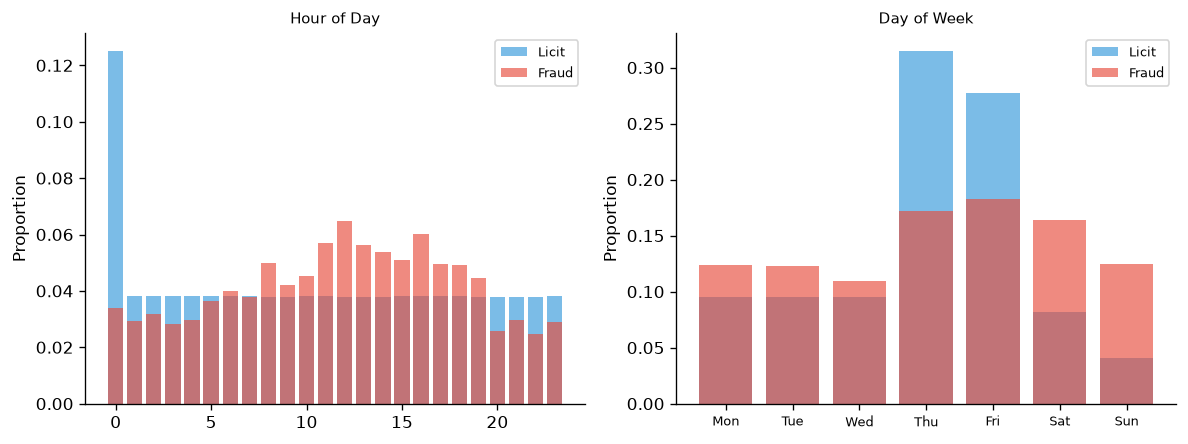
\includegraphics[width=0.8\textwidth]{IMG/hourday.png}
    \caption{IBM AMLSim hour and day of the week distributions}
    \label{fig:hourday}
\end{figure} 

Finally we take a look at the Node features. The only intresting one is \textit{Bank Name}, Figure \ref{fig:bank} shows the distribution of licit and illicit nodes over the 10 biggest banks.
\begin{figure}
    \centering
    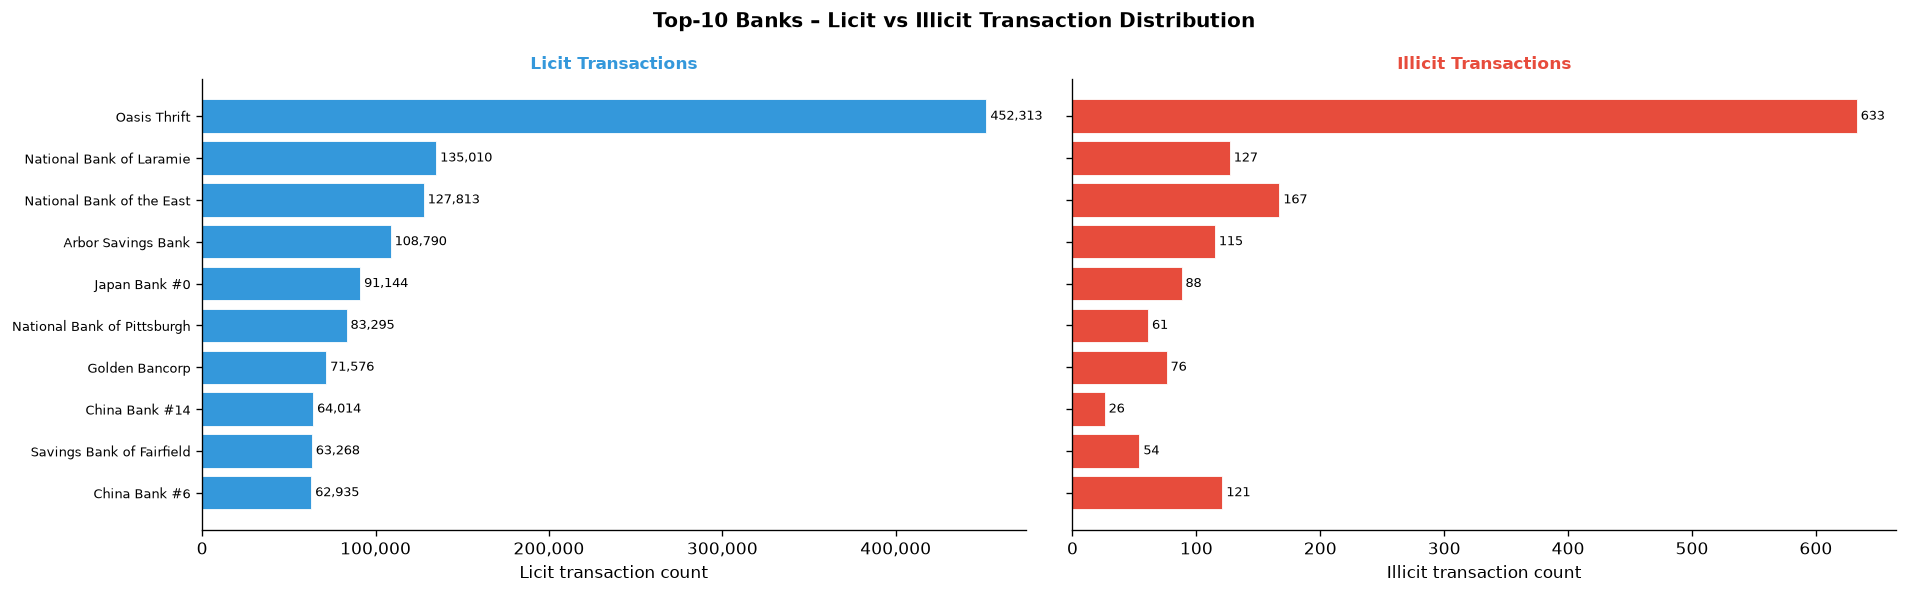
\includegraphics[width=0.8\textwidth]{IMG/banks.png}
    \caption{IBM AMLSim banks distribution}
    \label{fig:bank}
\end{figure} 
%--------------------------------------------------------------
% proposedModels.tex (use thesis.tex as main file)
%--------------------------------------------------------------
\chapter{Proposed Approach and Methodology}
%--------------------------------------------------------------

%--------------------------------------------------------------
% experiments.tex (use thesis.tex as main file)
%--------------------------------------------------------------
\chapter{Experiments}

\section{Experimental Settings}

\section{Hyperparameter Tuning}

\section{Experimental Results and Discussion}
%--------------------------------------------------------------

%--------------------------------------------------------------
% challenges.tex (use thesis.tex as main file)
%--------------------------------------------------------------
\chapter{Challenges}
%--------------------------------------------------------------

%--------------------------------------------------------------
% conclusion.tex (use thesis.tex as main file)
%--------------------------------------------------------------
\chapter{Conclusions}
%--------------------------------------------------------------



\section{Future Directions}
%--------------------------------------------------------------
\label{futureDirections}

% considerare timestamp
% IBM AMLSim Large per evitare overfitting in multiclass e consentire un modello piu grande
% provare piu iperparametri
%--------------------------------------------------------------
% futureDirections.tex (use thesis.tex as main file)
%--------------------------------------------------------------
\chapter{Future Directions}
%--------------------------------------------------------------
\label{futureDirections}

% considerare timestamp

%--------------------------------------------------------------
% Appendix
%--------------------------------------------------------------
\appendix
%--------------------------------------------------------------
% software.tex (use thesis.tex as main file)
%--------------------------------------------------------------
\chapter{Software}
%--------------------------------------------------------------
% spiego quale feature utilizzo

%--------------------------------------------------------------

\bibliographystyle{plain} % 
\bibliography{refs} % Entries are in the refs.bib file

%--------------------------------------------------------------
\end{document}
%--------------------------------------------------------------
